% The contents of this file will be inserted into the _Solutions version of the
% output tex document.  Here's an example:

% If assignment with subquestion (1.a) requires a written response, you will
% find the following flag within this document: <SCPD_SUBMISSION_TAG>_1a
% In this example, you would insert the LaTeX for your solution to (1.a) between
% the <SCPD_SUBMISSION_TAG>_1a flags.  If you also constrain your answer between the
% START_CODE_HERE and END_CODE_HERE flags, your LaTeX will be styled as a
% solution within the final document.

% Please do not use the '<SCPD_SUBMISSION_TAG>' character anywhere within your code.  As expected,
% that will confuse the regular expressions we use to identify your solution.

\def\assignmentnum{3 }
\def\assignmenttitle{XCS234 Assignment \assignmentnum}
\input{macros}
\begin{document}
\pagestyle{myheadings} \markboth{}{\assignmenttitle}

% <SCPD_SUBMISSION_TAG>_entire_submission

This handout includes space for every question that requires a written response.
Please feel free to use it to handwrite your solutions (legibly, please).  If
you choose to typeset your solutions, the |README.md| for this assignment includes
instructions to regenerate this handout with your typeset \LaTeX{} solutions.
\ruleskip

\LARGE
1.b
\normalsize

% <SCPD_SUBMISSION_TAG>_1b
\begin{answer}
  % ### START CODE HERE ###
  \begin{table}[h]
  \centering
  \begin{tabular}{ccc}
    \toprule
    IQL Expectile & Eval\_AverageReturn & Eval\_StdReturn \\
    \midrule
    $0.2$ & \textbf{
      -22.16
    } & \textbf{
      8.39
    } \\
    $0.9$ & \textbf{
      -19.67
    } & \textbf{
      5.94
    } \\
    \bottomrule
  \end{tabular}
  \label{table:Problem_1_b}
  \caption{Eval Average Return for different IQL Expectile value on PointmassEasy-v0}
  \end{table}

  \textbf{PointmassEasy-v0 IQL Zeta=0.2 Last Trajectory Plot}
  \begin{center}
  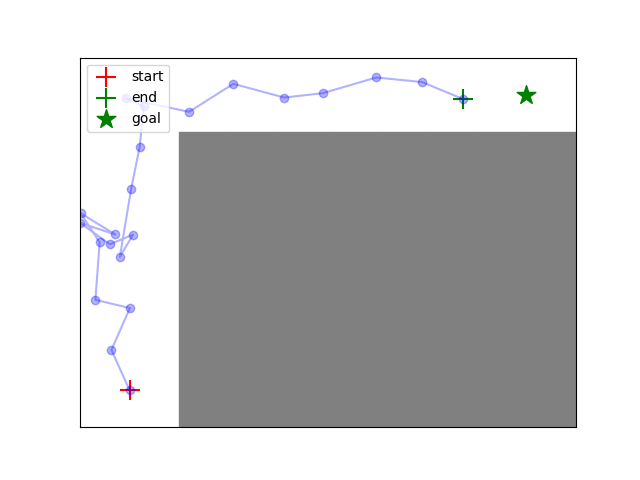
\includegraphics[width=0.85\textwidth]{figures/eval_last_traj_iql_easy_0.2.png}
  \end{center}

  \textbf{PointmassEasy-v0 IQL Zeta=0.9 Last Trajectory Plot}
  \begin{center}
  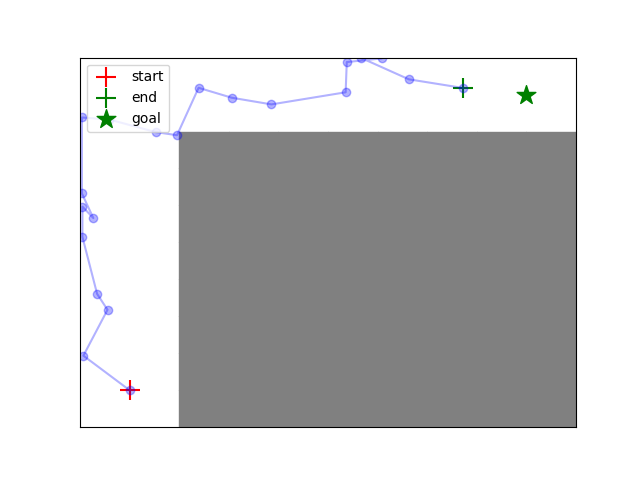
\includegraphics[width=0.85\textwidth]{figures/eval_last_traj_iql_easy_0.9.png}
  \end{center}

  Zeta of 0.9 outperforms zeta of 0.2. This makes sense because the stated goal of using an Expectile
  loss in the IQL paper is to predict an upper expectile of the TD targets that approximates the maximum
  of V(s). With zeta of 0.2 we put a weight of 0.2 on good actions which results in a pessimistic value of
  V(s) and therefore V(s) is too low and advantages A = Q - V are too high, so the actor can't distinguish
  good actions from bad actions because everything looks above average relative to V.

  Zeta of 0.9 does the opposite, predicting an optimistic V(s) for in-distribution actions, like the IQL paper
  intended, so the actor learns to up-weight the good in-distribution actions.

  % ### END CODE HERE ###
\end{answer}
% <SCPD_SUBMISSION_TAG>_1b
\clearpage

\LARGE
1.c
\normalsize

% <SCPD_SUBMISSION_TAG>_1c
\begin{answer}
  % ### START CODE HERE ###
  \begin{table}[h]
  \centering
  \begin{tabular}{cccc}
    \toprule
    IQL Expectile & Exploration & Eval\_AverageReturn & Eval\_StdReturn \\
    \midrule
    $0.2$ & \text{Random} & \textbf{
      -79.5
    } & \textbf{
      33.025
    } \\
    $0.2$ & \text{RND} & \textbf{
      -54.78
    } & \textbf{
      16.92
    } \\
    \bottomrule
  \end{tabular}
  \label{table:Problem_1_c}
  \caption{Eval Average Return for different exploration strategies on PointmassMedium-v0}
  \end{table}

  \textbf{PointmassMedium-v0 IQL Zeta=0.2 Random Last Trajectory Plot}
  \begin{center}
  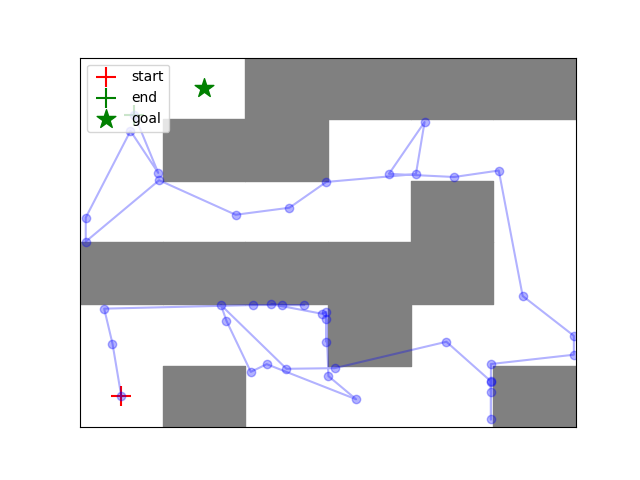
\includegraphics[width=0.85\textwidth]{figures/eval_last_traj_iql_medium_random.png}
  \end{center}

  \textbf{PointmassMedium-v0 IQL Zeta=0.2 RND Last Trajectory Plot}
  \begin{center}
  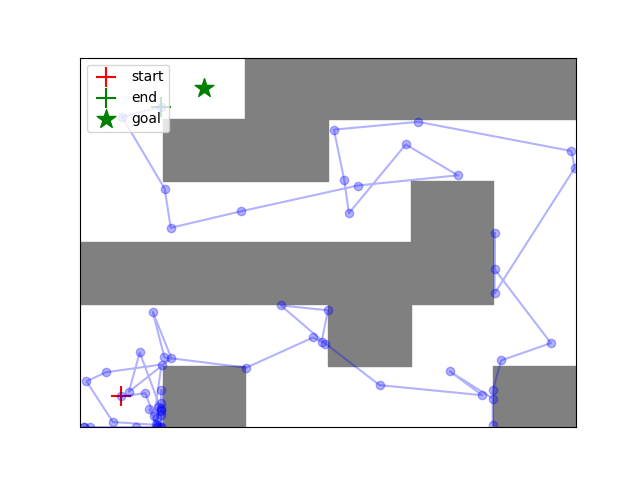
\includegraphics[width=0.85\textwidth]{figures/eval_last_traj_iql_medium_rnd.png}
  \end{center}

  The offline RL policy trained on the data produced by the RND exploration strategy outperformed
  the policy trained on the data produced by the Random exploration strategy. This tells us that a 
  data exploration strategy that actively seeks out novel states, rather than stumbling upon them
  randomly can build a better dataset for an offline RL policy.
  % ### END CODE HERE ###
\end{answer}
% <SCPD_SUBMISSION_TAG>_1c
\clearpage


\LARGE
2.b
\normalsize

% <SCPD_SUBMISSION_TAG>_2b
\begin{answer}
  % ### START CODE HERE ###
  % ### END CODE HERE ###
\end{answer}
% <SCPD_SUBMISSION_TAG>_2b
\clearpage

\LARGE
2.c
\normalsize

% <SCPD_SUBMISSION_TAG>_2c
\begin{answer}
  % ### START CODE HERE ###
  % ### END CODE HERE ###
\end{answer}
% <SCPD_SUBMISSION_TAG>_2c
\clearpage

% <SCPD_SUBMISSION_TAG>_entire_submission

\end{document}
